\documentclass[11pt]{beamer}
\usepackage{verbatim}
\usepackage{amsmath}
\usepackage{amsthm}
\usepackage{graphics}
\usepackage{multicol}
\usepackage{color}
\usepackage{stmaryrd}
\usefonttheme[onlymath]{serif}

\title{Progess Report 7}
\date{\today}
\author{Xie Li}
\begin{document}
\maketitle

\begin{frame}\frametitle{Overview of the Progress}
\begin{itemize}
\item Continue the development of the tool with Weizhi. Current progress:
\item Continue the development with Weizhi.
\item Currently implemented the checking of \textbf{path feasibility}, LTLf: $\mathbf{G}p$ and LTLf: $\textbf{F}p$.
\end{itemize}

\end{frame}


\begin{frame}\frametitle{Current Core Algorithm}

\begin{center}
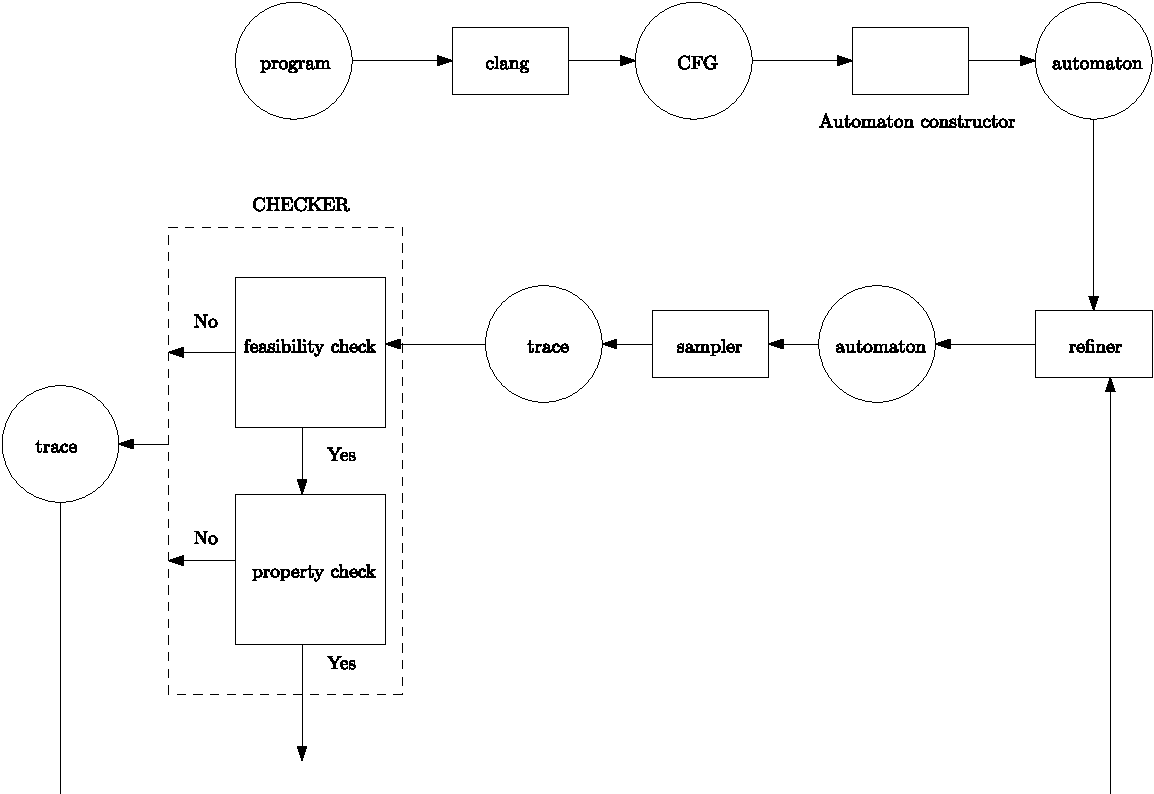
\includegraphics[scale=0.5]{flowgraph.pdf}
\end{center}

\end{frame}

\begin{frame}\frametitle{Test case}
%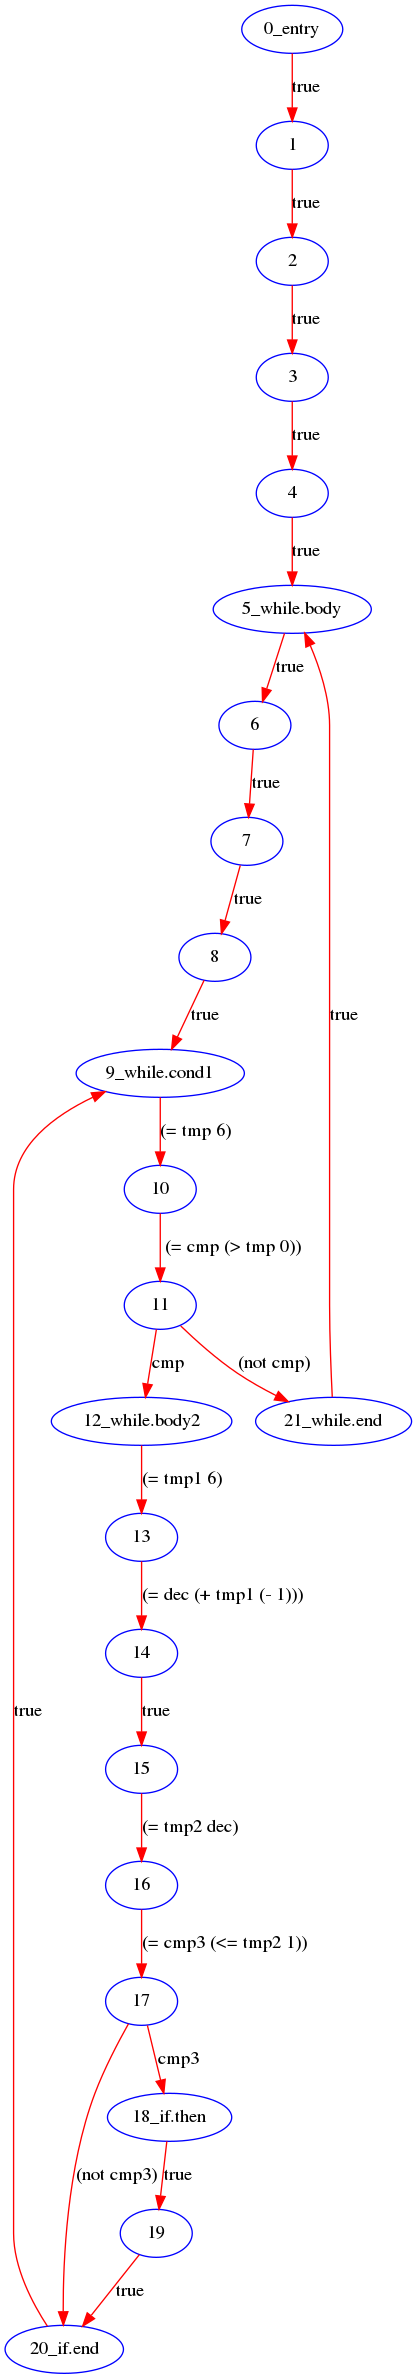
\includegraphics[scale=0.2]{cfa.png}
\begin{center}
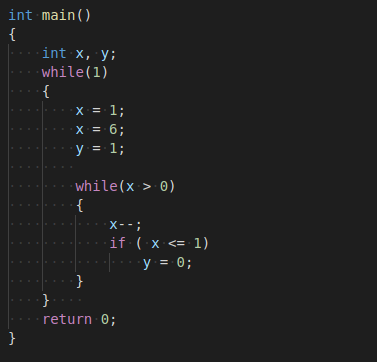
\includegraphics[scale=0.6]{pro.png}
\end{center}
\end{frame}

\begin{frame}\frametitle{Path Feasibility}

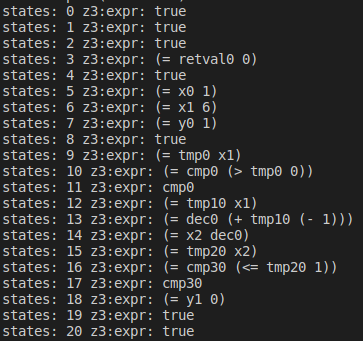
\includegraphics[scale=0.4]{p1.png}
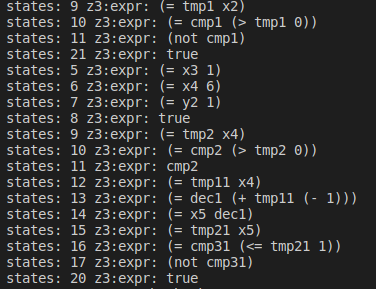
\includegraphics[scale=0.4]{p2.png}

Not feasible.
\end{frame}

\begin{frame}\frametitle{Path Feasibility}
\begin{center}
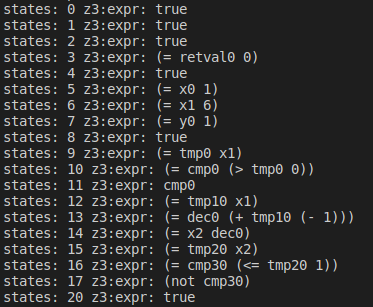
\includegraphics[scale=0.4]{p4.png}
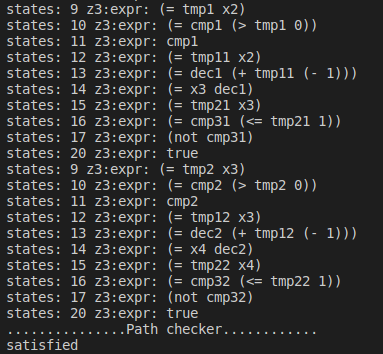
\includegraphics[scale=0.4]{p5.png}
\end{center}
\end{frame}


\begin{frame}\frametitle{LTLf: $\mathbf{F}(x > 1)$}

\begin{itemize}
\item Use a map to store pair $\langle a, x > 0\rangle$
\item 
The formula is given by $\mathbf{F}a$ and will be parsed by spot into an AST.
\item Then we can extract the name of $a$ and use a map to restore $x > 0$.
\item Substitute the occurence of $x$ with $x_1, x_2, \ldots$ along the path and do the checking.
\end{itemize}

\end{frame}

\begin{frame}\frametitle{LTLf: $\mathbf{F}(x > 1)$}

\begin{center}
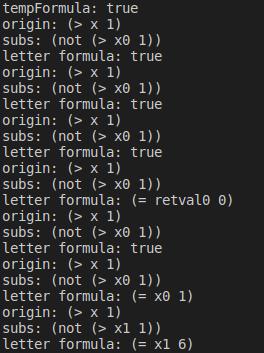
\includegraphics[scale=0.6]{fx>1.png}
\end{center}

\end{frame}

\begin{frame}\frametitle{Sample Based Checker}

Repeat the sampling and the checking several times.

\end{frame}

\end{document}